\subsubsection{Leverage}
	\begin{twoColTable}
		\hline
		\textbf{Description}
			& A data point with high leverage has a dangerous influence on the regression model because it can significantly falsify the results.\\
		\hline
		\textbf{Expected value of the Leverage statistic}
			& $\mathrm{E}(h_i) = \frac{p+1}{n}$\\
		\hline
		Number of predictor variables
			& $p$\\
		\hline
		Number of measurements
			& $n$\\
		\hlijne
		Interpretation of leverage statistic
			& If an observation has a leverage statistic $h_i >> \mathrm{E}(h_i)$ it is considered to have high leverage and a dangerous influence in the model.\\
		\hline	
		\textbf{Cook's Distance}
			& 	$d_i = \frac{h_i}{1-h_i}\frac{\tilde{r}^2_i}{p+1}$\\
		\hline
		Interpretation of Cook's Distance
			& A value $d_i > 1$ must be considered as dangerous.\\
		\hline
	\end{twoColTable}
	
	\RCode
	{
		Leverage Plots
	}
	{
		sections/RegressionAnalysis/ResidualAnalysis/DiagnosticsInstruments/Leverage/Leverage.R
	}
	
	\begin{figure}[H]\centering
		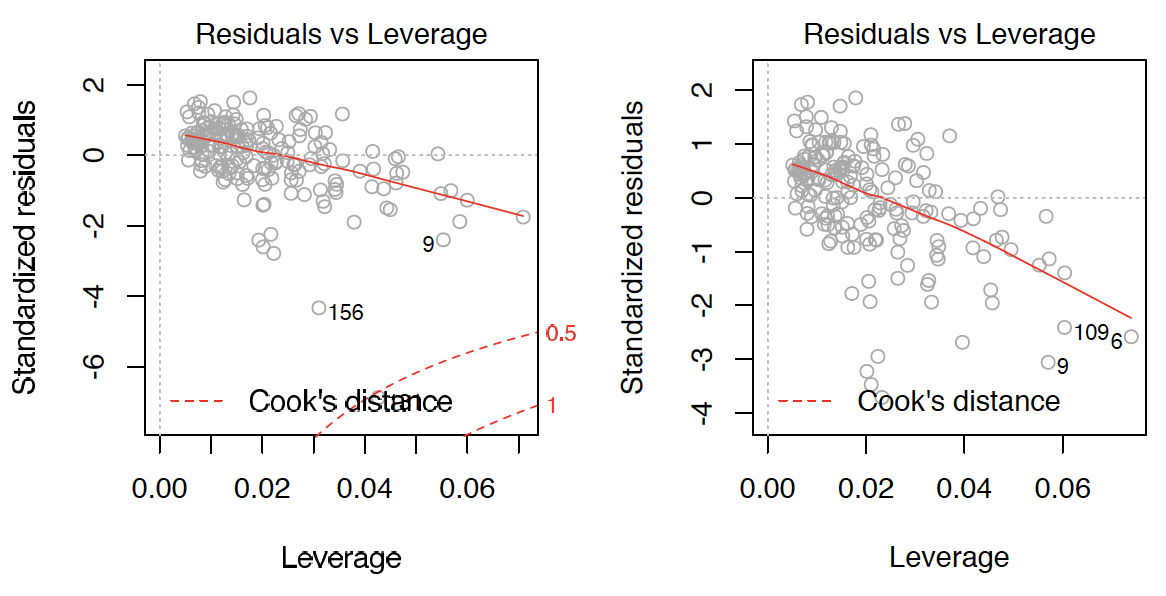
\includegraphics[width=0.7\linewidth]{images/Leverage.png}
		\caption{Leverage plots: Leverage vs standardized residuals and Cook's distance displayed.\newline Left: complete data, Right: High leverage points 131 and 156 were removed from the data set}
	\end{figure}